%   Section: "PMFs"  (JC & Conner)
%      -notable asymmetry across the membrane center (focus on urea)
%      -effect of making the US PMFs symmetric using g_wham, along with autocorrelation time estimates
%      -longer equilibration makes US converge more quickly
%      -comparison using data from z = (0,36) @ 20 ns/window vs. z = (-36,36) @ 10 ns/window

\subsection{Potentials of Mean Force}
  \par In the solubility-diffusion model, the PMF is a critical component of the permeability (see Eq.~\ref{eq:solubility-diffusion}).  Given its exponential weighting, the PMF may even be considered the greatest contributor to the permeability, making its accurate calculation of paramount importance.  To determine the best approach for calculating the PMF, we have compared four methods mentioned earlier and investigated the appropriate balance between equilibration time and sampling time.

\begin{figure}[htbp]
\begin{center}
	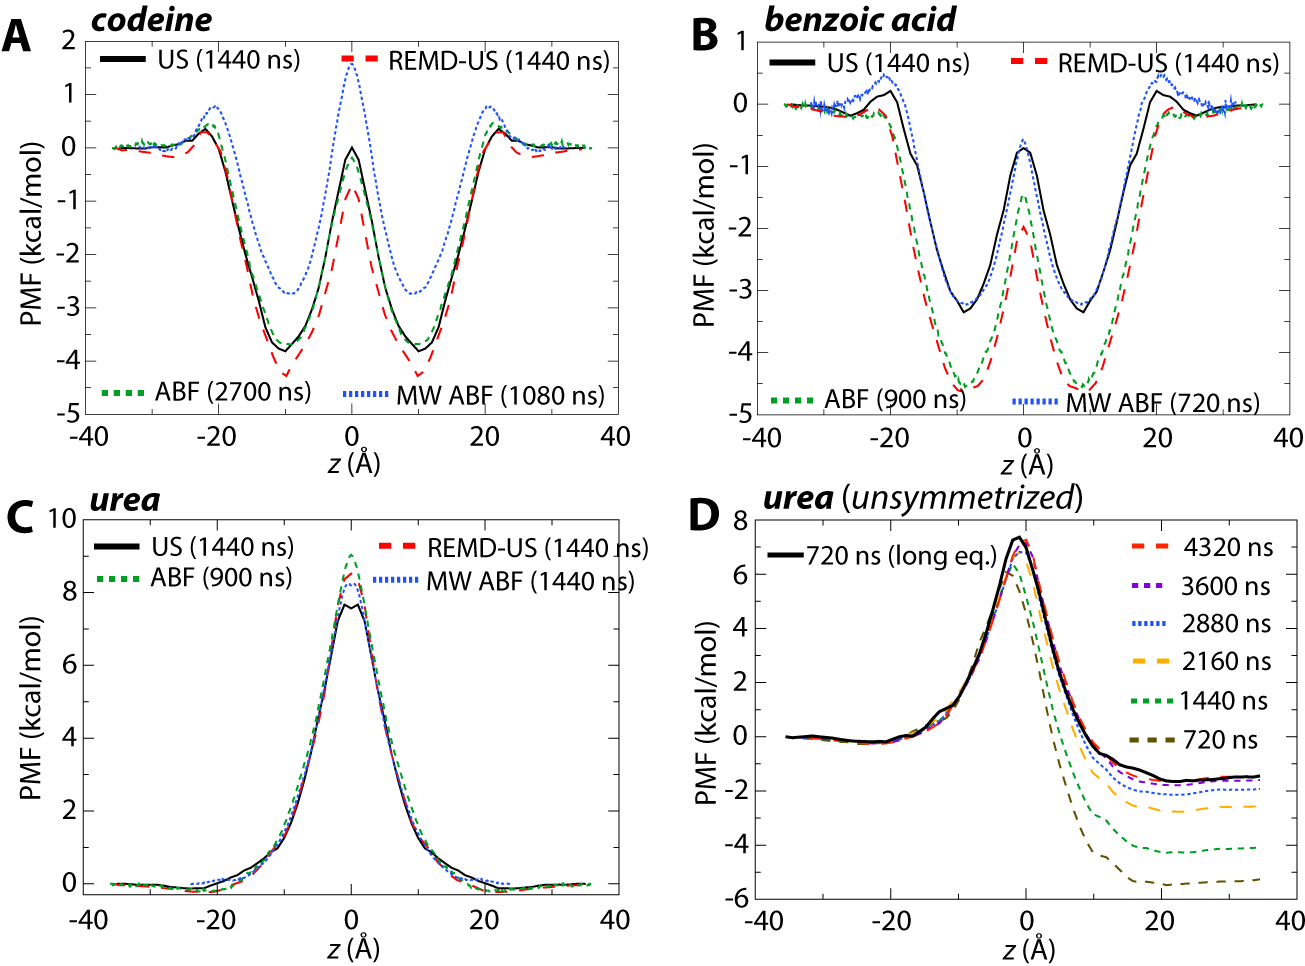
\includegraphics[width=0.8\textwidth]{Figures/PMFs-all}
	\caption{Potentials of Mean Force (PMFs) for the permeants (A) codeine, (B) benzoic acid, and (C) urea.  In each case, four PMFs from each of the methods are given: US (black, solid), REUS (red, large dashes), ABF (green, medium dashes) and MW-ABF (blue, small dashes).  All PMFs have been symmetrized about the membrane center.  (D) Convergence of the unsymmetrized PMF for urea.  PMFs determined using REUS for a total simulation time of 720\,ns -- 4.3\,$\mu$s are shown as various colored, dashed lines.  The PMF determined after 500\,ns of total equilibration and 720\,ns of sampling is also shown (solid black line) and is comparable to that from 4.3\,$\mu$s of sampling with less equilibration. See Fig.~S1 for the unsymmetrized PMFs for codeine and benzoic acid.}
	\label{fig:PMFs}
\end{center}
\end{figure}

  \par The PMFs were determined by bringing the permeant across the entire membrane and then symmetrizing the resulting profile, {\it i.e.}, the profiles were adjusted to be identical on either side of the membrane center and to both start and end at 0.  The resulting {\it symmetrized} PMFs for all three permeants are shown in Fig.~\ref{fig:PMFs}A-C.  Each plot shows varying levels of disagreement between the methods, although no method is consistently different.  For example, while for codeine, ABF and US are in agreement and MW-ABF is the most discrepant, for benzoic acid, MW-ABF and US are in agreement but different from REUS and ABF.  Thus, it is not apparent from these three permeants that any one method for determining the PMF converges more rapidly than the others.

  \par The original profiles, prior to symmetrization, reveal a disturbing degree of asymmetry, and therefore accumulated error.  The evolving {\it unsymmetrized} profiles for urea are shown in Fig.~\ref{fig:PMFs}D {\color{red} and for codeine and benzoic acid in Fig.~S1}.  After 720\,ns (10\,ns/window), the asymmetry between the two end points is $\sim$5\,kcal/mol.  This asymmetry decreases at a rate of only 1\,kcal/mol per 720\,ns, and still persists at $\sim$1.5\,kcal/mol after over 4\,$\mu$s of sampling. Trajectory snapshots from US of codeine bowing the interfacial phosphates as well as urea coordinating waters at the membrane core are shown in Fig.~S2 and S3, respectively, highlighting potentially slow converging orthogonal degrees of freedom.

  \par One reason for the growing error in the PMF as the permeant goes through the membrane is the residual disturbance to the membrane structure from the steered MD used to generate the starting states. The time blocked probability distributions of headgroup phosphates and water in the vicinity of urea (shown in Fig.~S4) support the existence of non-equilibrium artifacts. One way to ameliorate this disturbance is longer equilibration of the starting states.  As a test of this idea, selected starting states for urea were equilibrated for a particular amount of time, dependent on their distance from the membrane center, namely 100\,ns at the center; 50\,ns at
%+/-5\,\AA, +/-10\,\AA, and +/-15\,\AA; 25\,ns at +/-20\,\AA; 15\,ns at +/-25\,\AA; and 10\,ns at +/-30\,\AA,
  $\pm$5\,\AA, $\pm$10\,\AA, and $\pm$15\,\AA; 25\,ns at $\pm$20\,\AA; 15\,ns at $\pm$25\,\AA; and 10\,ns at $\pm$30\,\AA,
  giving a total of 500\,ns of equilibration.  Intermediate windows at each \aa ngstrom were then generated from these equilibrated states.  The unsymmetrized PMF resulting from 720\,ns of sampling with REUS is shown as the solid black line in Fig.~\ref{fig:PMFs}D.  It is immediately apparent that this newly generated PMF and its asymmetry after only 720\,ns are comparable to those after 4.3\,$\mu$s of sampling without sufficient equilibration.
 Thus,
 %one must take care when generating the starting states to avoid significant residual non-equilibrium effects from persisting during production sampling.
 starting states should be sufficiently equilibrated in order to avoid artifacts resulting from their initial setup, {\color{red} in agreement with earlier recommendations by Palonc{\'{y}}ov{\'{a}} et al.~\cite{Paloncyova2012}.}

% talk about alternatives to SMD in the discussion

% win0: 100 ns
% win+/-5: 50 ns
% win+/-10: 50 ns
% win+/-15: 50 ns
% win+/-20: 25 ns
% win+/-25: 15 ns
% win+/-30: 10 ns

%10.0 9.4 8.5 8.0  8.25 (60 ns)

  \par In the preceding calculations, we determined the PMF for the entire permeation process, i.e., from $z=36$\,\AA~to $-36$\,\AA, after which the resulting PMF was symmetrized about the membrane center.  However, noting the expectation of a symmetric PMF, for many published cases the PMF is only determined from $z=36$ to 0\,\AA~\cite{Marrink1996,Bemporad2004,Holland2012}.  Given a finite amount of time for sampling, one may ask which is better --- to sample the full range of permeation for time $t$ or to sample half of the range for time $2t$ and then mirror it across the membrane center?  These two possibilities are compared in Fig.~S5.  When considering the {\it unsymmetrized} PMF from 10\,ns/window of the full range (10\,ns $\times$ 72 windows), the maximum value of 10.0\,kcal/mol is a full 1.8\,kcal/mol greater than the (presumably) converged result from 60\,ns/window (8.3\,kcal/mol).  For 20\,ns/window over half of the range (20\,ns $\times$ 36 windows), the maximum in the PMF is 9.4\,kcal/mol, apparently a better result than simulating over the full range.  However, once the result over the full range is symmetrized, the peak shifts to 8.0\,kcal/mol, significantly closer to the final result than the half-range peak.  Thus, the combination of simulating over the entire range along with the requirement of symmetrization appears to produce a more accurate result than simulating over half of the range for twice as long.
